\documentclass[9.5pt]{article}
\usepackage[utf8]{inputenc}
\usepackage[english]{babel}
\usepackage{cvstyle}

\begin{document}

% ---------- Header ----------
\noindent
\begin{minipage}[c]{0.78\textwidth}
  \cvname{Varoujan KARAKOZIAN}\\[2pt]
  \cvrole{AI Engineer Apprentice --- Dassault Systèmes}\\[4pt]
  {\small
    +33~7~81~78~53~77 ~~\textbullet~~
    \href{mailto:Varoujan.Karakozian@efrei.net}{Varoujan.Karakozian@efrei.net} ~~\textbullet~~
    3 rue des Œillets, 94140 Alfortville, France ~~\textbullet~~
    Born 3 Nov 2005
  }
\end{minipage}%
\hfill
\begin{minipage}[c]{0.15\textwidth}
  \raggedleft
  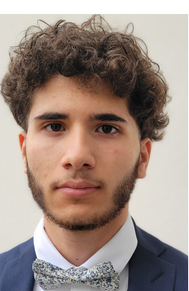
\includegraphics[width=1.85cm]{photo.png}
\end{minipage}

\vspace{2pt}
{\color{accent}\rule{\linewidth}{1.1pt}}
\vspace{2pt}

% ---------- Two-column body ----------
\noindent
\begin{minipage}[t]{0.645\textwidth}

\section*{\large\bfseries\color{accent}Profile}
\vspace{-2pt}
\noindent\small
Second-year engineering student at EFREI Paris, specializing in \textbf{Big Data \& Machine Learning (BDML)}. Currently on a three-year work-study program (2025--2028) with \textbf{Dassault Systèmes}, in an R\&D DevSecOps team building AI tooling for internal developers, working with \textbf{MCP} and \textbf{RAG}.

\section*{\large\bfseries\color{accent}Education}
\vspace{-2pt}
\cventry{Engineering Cycle --- Big Data \& Machine Learning specialization}{EFREI Paris (work-study)}{2025 -- 2028}
{\small 2nd year in progress.}

\vspace{2pt}
\cventry{International Preparatory Classes (English track)}{EFREI Paris}{}

\vspace{2pt}
\cventry{Baccalauréat (French high-school diploma), High Honors}{Lycée Sainte-Marie, Créteil}{}

\section*{\large\bfseries\color{accent}Experience}
\vspace{-2pt}
\cventry{AI Engineer Apprentice}{Dassault Systèmes --- Vélizy-Villacoublay, France}{Sept. 2025 -- Jun 2028}
\begin{itemize}\small
  \item Built \textbf{MCP} (Model Context Protocol) tools connecting an AI coding assistant to internal systems: automatic version-control context detection, build metadata retrieval, automated web-scraping data collection (Selenium).
  \item Designed and evaluated a local \textbf{RAG} pipeline (BM25) for internal documentation indexing, replacing an LLM-based approach that was 2--3 orders of magnitude slower and more token-expensive.
  \item Built a three-model evaluation protocol (question generation, answering, LLM-as-judge) measuring retrieval Accuracy@K across roughly 8,500 questions over 3 benchmark corpora.
  \item Contributed to \textbf{FixGen}, a generative-AI crash diagnosis tool: built data-collection tools (URL classification, automated stack-trace scraping).
\end{itemize}

\vspace{1pt}
\cventry{Sales Internship}{Lacoste --- Créteil, France}{2025 (1 month)}
\begin{itemize}\small
  \item Welcomed and advised customers, providing personalized recommendations tailored to their needs.
  \item Used language skills (English, Spanish) to assist international customers.
\end{itemize}

\vspace{1pt}
\cventry{Warehouse Internship --- Order Picker}{Phoenix Pharma --- Créteil, France}{2024 (1 month)}
\begin{itemize}\small
  \item Logistics: preparing and checking pharmaceutical orders.
  \item Teamwork: effective collaboration with warehouse teams in a fast-paced environment.
\end{itemize}

\section*{\large\bfseries\color{accent}Academic Projects}
\vspace{-2pt}
\cvproject{NYC Taxi --- Data Visualization \& Business Intelligence}{2026}
\begin{itemize}\small
  \item Exploratory analysis of NYC taxi trips (Python, Pandas, Plotly, Streamlit): data cleaning, interactive visualizations, BI dashboard with KPIs.
\end{itemize}

\vspace{1pt}
\cvproject{Wine Quality Classification --- Machine Learning}{2026}
\begin{itemize}\small
  \item Compared multiple models (Random Forest, SVM, etc.) to predict wine quality from physicochemical features.
\end{itemize}

\vspace{2pt}
\noindent\small
\textbf{Earlier projects ---}
\textbf{Climate Change Data Analysis} (2025): full PCA pipeline showing a correlation between inequality and national pollution.
\textbf{Voll'Effrei} (2025): volleyball video game, interdisciplinary physics/CS project.
\textbf{Intelligent Chatbot} (2024): Python chatbot based on TF-IDF analysis.
\textbf{CDataFrame} (2024): a C-language DataFrame inspired by Pandas.

\end{minipage}%
\hfill
\begin{minipage}[t]{0.305\textwidth}

\section*{\large\bfseries\color{accent}Skills}
\vspace{-2pt}
\small
\textbf{AI / Machine Learning}
\begin{itemize}
  \item MCP (Model Context Protocol)
  \item RAG \& RAG evaluation
  \item LLM-as-judge, Accuracy@K
  \item BM25, scikit-learn (Random Forest, SVM)
\end{itemize}
\vspace{2pt}
\textbf{Programming}
\begin{itemize}
  \item Python, C, Java
\end{itemize}
\vspace{2pt}
\textbf{Tools \& platforms}
\begin{itemize}
  \item Git/GitHub, Linux
  \item Selenium, Streamlit, Plotly, Pandas
\end{itemize}
\vspace{2pt}
\textbf{Databases}
\begin{itemize}
  \item SQL, MySQL, SQLite
\end{itemize}
\vspace{2pt}
\textbf{Soft skills}
\begin{itemize}
  \item Teamwork
  \item Adaptability
  \item Self-taught
  \item Initiative
  \item Creative
  \item Autonomous
  \item Versatile
\end{itemize}

\section*{\large\bfseries\color{accent}Languages}
\vspace{-2pt}
\small
\begin{itemize}
  \item French --- Native
  \item English --- Advanced (B2)
  \item Armenian --- Intermediate (B1)
  \item Spanish --- Intermediate (B1)
\end{itemize}

\section*{\large\bfseries\color{accent}Hobbies}
\vspace{-2pt}
\small
\begin{itemize}
  \item Music
  \item Climbing
  \item Chess
  \item Basketball
\end{itemize}

\end{minipage}

\end{document}
